\documentclass[a4paper]{article}
\usepackage[
	pdftex,
	colorlinks=true,
	bookmarksnumbered=true,
	bookmarksopen=true,
	bookmarksopenlevel=3,
	pdfstartview=FitP,
	urlcolor=blue,
]{hyperref}
\pdfinfo{
	/Title(Esercitazione di Laboratorio: Amplificatori operazionali con retroazione)
	/Author(Coa Giulio, Licastro Dario, Montano Alessandra)
}
\usepackage[italian]{babel}
\usepackage{geometry,titling,mdsymbol,stmaryrd,graphicx,subcaption,amsmath}
\graphicspath{{./Image/}}
\renewcommand\maketitlehooka{
	\null
	\mbox{}
	\vfill
}
\renewcommand\maketitlehookd{
	\vfill
	\null
}
\title{
	\begin{center}
		Esercitazione di Laboratorio:
	\end{center}
	\newline
	\begin{center}
		Amplificatori operazionali con retroazione
	\end{center}
}
\author{
	Coa Giulio
	\and
	Licastro Dario
	\and
	Montano Alessandra
}
\begin{document}
	%-----------------------------------------------------------------------------
	%  TITLE
	%-----------------------------------------------------------------------------
	\begin{titlingpage}
		\maketitle
	\end{titlingpage}
	\newpage
	%-----------------------------------------------------------------------------
	%  PURPOSE OF THE EXPERIENCE
	%-----------------------------------------------------------------------------
	\section{Scopo dell'esperienza}
	Gli scopi di questa esercitazione sono:
	\begin{itemize}
		\item Analizzare il comportamento e misurare i parametri di amplificatori reazionati.
		\item Verificare alcune deviazioni rispetto al comportamento previsto con i modelli ideali.
	\end{itemize}
	%-----------------------------------------------------------------------------
	%  INSTRUMENTATION USED
	%-----------------------------------------------------------------------------
	\section{Strumentazione utilizzata}
	La strumentazione usata durante l'esercitazione è:
	\begin{center}
		\begin{tabular}{ |c|c|c| }
			\hline
			\multirow{\textbf{Strumento}}	 & \textbf{Marca e Modello} & \textbf{Caratteristiche} \\
			\hline
			\multirow{Oscilloscopio}		 & Rigol DS1054Z			& 4 canali, \\
											 &							& $ B = 50 \, \mathrm{MHz} $, \\
											 &							& $ f_{\mathrm{c}} = 1 \, \mathrm{G\frac{Sa}{s}} $, \\
											 &							& $ R_{\mathrm{i}} = 1 \, \mathrm{M\Omega} $, \\
											 &							& $ C_{\mathrm{i}} = 13 \, \mathrm{pF} $, \\
											 &							& $ 12 \, \mathrm{Mbps} $ di profondità di memoria \\
			\multirow{Generatore di segnali} & Rigol DG1022				& 2 canali, \\
											 &							& $ f_{\mathrm{uscita}} = 20 \, \mathrm{MHz} $, \\
											 &							& $ Z_{\mathrm{uscita}} = 50 \, \mathrm{\Omega} $ \\
			\multirow{Alimentatore in DC}	 & Rigol DP832				& 3 canali \\
			\multirow{Scheda premontata}	 & A3						& \\
			\multirow{Cavi coassiali}		 &							& Capacità dell'ordine dei $ 80 \div 100 \, \mathrm{p\frac{F}{m}} $ \\
			\multirow{Connettori}			 &							& \\
			\hline
		\end{tabular}
	\end{center}
	%-----------------------------------------------------------------------------
	%  THEORETICAL PREMISES
	%-----------------------------------------------------------------------------
	\section{Premesse teoriche}
		\subsection{Incertezza sulla misura dell'oscilloscopio}
			La misura del valore di un segnale tramite l’oscilloscopio (sia esso l'ampiezza, la frequenza, il periodo, etc.) presenta un'incertezza che dipende, principalmente, da due fattori:
			\begin{itemize}
				\item l’incertezza strumentale introdotta dall’oscilloscopio (ricavabile dal manuale).
				\item l’incertezza di lettura dovuta all’errore del posizionamento dei cursori.
			\end{itemize}
			Quest’ultima incertezza deriva dal fatto che il segnale visualizzato non ha uno spessore nullo sullo schermo.
		\subsection{Amplificatore}
			Un amplificatore è un doppio bipolo unidirezionale caratterizzato dalla seguente relazione
			\begin{center}
				$ y(t) = A \cdot x(t) $
			\end{center}
			\newline
			Dove $ A $ è detto guadagno dell'amplifiatore.
			\begin{figure}[h!]
				\centering
				\begin{subfigure}{0.4\textwidth}
					\centering
					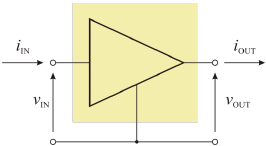
\includegraphics[scale=0.7]{amplificatore}
					\caption{Amplificatore.}
				\end{subfigure}
				\begin{subfigure}{0.4\textwidth}
					\centering
					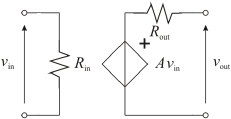
\includegraphics[scale=0.7]{amplificatoreCircuito}
					\caption{Circuito equivalente ad un amplificatore.}
				\end{subfigure}
				\label{fig:amplificatore}
			\end{figure}
			\newpage
			In base al tipo di segnale in ingresso e in uscita, possiamo distinguere quattro tipi di amplifiatori:
			\begin{itemize}
				\item Amplificatore di Tensione.
				\item Amplificatore di Transconduttanza.
				\item Amplificatore di Transresistenza.
				\item Amplificatore di Corrente.
			\end{itemize}
			\subsubsection{Amplificatore operazionale}
				L'amplificatore operazionale è un amplificatore differenziale, ovvero amplifica la differenza delle tensioni ai suoi capi, che presenta un'amplificazione $ A_{\mathrm{d}} $ idealmente infinita.
				\begin{equation*}
					\begin{split}
						A_{\mathrm{d}} &= \frac{v_{\mathrm{out}}}{v_{\mathrm{d}}} = \\
									   &= \frac{v_{\mathrm{out}}}{v^{+} - v^{-}}
					\end{split}
				\end{equation*}
				\begin{figure}[h!]
					\centering
					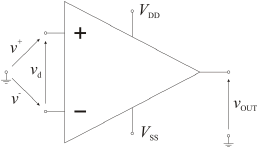
\includegraphics[scale=0.7]{amplificatoreOperazionale}
					\caption{Amplificatore operazionale.}
					\label{fig:amplificatoreOperazionale}
				\end{figure}
			\subsubsection{Amplificatore differenziale}
				L'amplificatore differenziale è un amplificatore che fornisce, in uscita, un segnale proporzionale alla differenza rispetto ai segnali in ingresso; esso caratterizzato dalle seguenti relazioni
				\begin{center}
					$ R_{\mathrm{in, v^{+}}} = R_{\mathrm{a}} + R_{\mathrm{b}} $
				\end{center}
				\newline
				\begin{center}
					$ R_{\mathrm{in, v^{-}}} = R_{\mathrm{b}}^{'} $
				\end{center}
				\newline
				\begin{center}
					$ R_{\mathrm{out}} = 0 $
				\end{center}
				\newline
				\begin{center}
					$ \frac{R_{\mathrm{a}}^{'}}{R_{\mathrm{b}}^{'}} = \frac{R_{\mathrm{a}}}{R_{\mathrm{b}}} \cdot (1 + \epsilon) $
				\end{center}
				\newline
				\begin{equation*}
					\begin{split}
						v_{\mathrm{out}} &= A_{\mathrm{diff}} \cdot v_{\mathrm{d}} - A_{\mathrm{cm}} \cdot v_{\mathrm{cm}} = \\
										 &= (\frac{R_{\mathrm{a}}}{R_{\mathrm{b}}} - \frac{R_{\mathrm{a}}}{R_{\mathrm{a}} + R_{\mathrm{b}}} \cdot \frac{\epsilon}{2}) \cdot v_{\mathrm{d}} - \frac{R_{\mathrm{a}}}{R_{\mathrm{a}} + R_{\mathrm{b}}} \cdot \epsilon \cdot v_{\mathrm{cm}} = \\
										 &\approx \frac{R_{\mathrm{a}}}{R_{\mathrm{b}}} \cdot v_{\mathrm{d}} - \frac{R_{\mathrm{a}}}{R_{\mathrm{a}} + R_{\mathrm{b}}} \cdot \epsilon \cdot v_{\mathrm{cm}}
					\end{split}
				\end{equation*}
				\begin{center}
					$ \mathrm{CMRR} = \frac{A_{\mathrm{diff}}}{A_{\mathrm{cm}}} \approx \frac{1}{\epsilon} \cdot (1 + A_{\mathrm{diff}}) $
				\end{center}
				\newline
				Dove $ \mathrm{CMRR} $ è il Common-Mode Rejection Ratio, $ A_{\mathrm{diff}} $ è l'amplificazione differenziale e $ A_{\mathrm{cm}} $ è l'amplificazione di modo comune.
				\begin{figure}[h!]
					\centering
					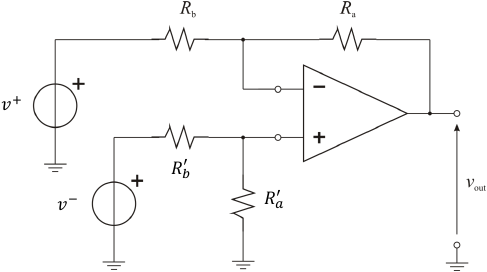
\includegraphics[scale=0.7]{amplificatoreDifferenziale}
					\caption{Amplificatore differenziale.}
					\label{fig:amplificatoreInvertente}
				\end{figure}
	%-----------------------------------------------------------------------------
	%  LABORATORY EXPERIENCE
	%-----------------------------------------------------------------------------
	\section{Esperienza in laboratorio}
		\subsection{Amplificatore non invertente}
			Abbiamo realizzato il circuito richiesto, collegando il modulo A3-1:
			\begin{itemize}
				\item Il generatore di segnali al connettore coassiale J3.
				\item L'alimentatore duale viene connesso, in modalità tracking, al morsetto \textbf{nomeMorsetto}.
				\item L'oscilloscopio, tramite due cavi coassiali BNC-coccodrillo, all'ingresso e all'uscita del circuito, rispettivamente gli ancoraggi J4 e J7 (massa) e J2 e J8 (massa).
			\end{itemize}
			E posizionando gli interruttori seguendo la seguente tabella
			\begin{center}
				\begin{tabular}{ |c|c|c| }
					\hline
					\multirow{\textbf{Interruttore}} & \textbf{Posizione} & \textbf{Note} \\
					\hline
					\multirow{S1}		     		 & 1				  & aperto \\
					\multirow{S2}		     		 & 2				  & chiuso \\
					\multirow{S4}		     		 & 2				  & chiuso \\
					\multirow{S5}		     		 & 1				  & aperto \\
					\multirow{S6}		     		 & 1				  & aperto \\
					\hline
				\end{tabular}
			\end{center}
			Abbiamo impostato $ V_{\mathrm{pp}} = 1 \, \mathrm{V} $ e $ f = 2 \, \mathrm{kHz} $, in seguito abbiamo misurato con l'oscilloscopio $ V_{\mathrm{i}} $ e $ V_{\mathrm{u}} $.
		\subsection{Amplificatore invertente}
			.
		\subsection{Amplificatore differenziale}
			.
		\subsection{Amplificatore AC/DC}
			.
	%-----------------------------------------------------------------------------
	%  RESULTS
	%-----------------------------------------------------------------------------
	\section{Risultati}
		\subsection{Amplificatore non invertente}
			Dai calcoli abbiamo ricavato che
			\begin{equation*}
				\begin{split}
					A_{\mathrm{v}} &= \frac{A_{\mathrm{d}}}{1 + \beta \cdot A_{\mathrm{d}}} = \\
								   &= \frac{A_{\mathrm{d}}}{1 + \frac{R_{2}}{R_{1} + R_{2}} \cdot A_{\mathrm{d}}} = \\
								   &= \frac{200k}{1 + \frac{12k}{100k + 12k} \cdot 200k} = \\
								   &= 9.33
					\end{split}
			\end{equation*}
			\begin{equation*}
				\begin{split}
					R_{\mathrm{in}} &= (R_{\mathrm{id}} + R_{1} \parallel R_{2}) \cdot (1 + A_{\mathrm{d}} \cdot \frac{R_{2} \parallel R_{\mathrm{id}}}{R_{2} \parallel R_{\mathrm{id}} + R_{1}}) = \\
									&= (1M + 100k \parallel 12k) \cdot (1 + 200k \cdot \frac{12k \parallel 1M}{12k \parallel 1M + 100k}) = \\
									&= 21.4 \, \mathrm{G\Omega}
				\end{split}
			\end{equation*}
			\begin{equation*}
				\begin{split}
					R_{\mathrm{out}} &= \frac{R_{\mathrm{o}}}{1 + \beta \cdot A_{\mathrm{d}}} \parallel (R_{1} + R_{2}) = \\
									 &= \frac{R_{\mathrm{o}}}{1 + \frac{R_{2}}{R_{1} + R_{2}} \cdot A_{\mathrm{d}}} \parallel (R_{1} + R_{2}) = \\
									 &= \frac{100}{1 + \frac{12k}{100k + 12k} \cdot 200k} \parallel (100k + 12k) = \\
									 &= 4.67 \, \mathrm{m\Omega}
				\end{split}
			\end{equation*}
			\newline
			\begin{center}
				\begin{tabular}{ |c|c|c|c|c| }
					\hline
					\multirow{\textbf{S3}} & \textbf{S7} & \textbf{$ V_{\mathrm{i}} $ [$ \mathrm{V} $]} & \textbf{$ V_{\mathrm{u}} $ [$ \mathrm{V} $]} & \textbf{$ A_{\mathrm{v}} $} \\
					\hline
					\multirow{1}		   & 1			 & $ 1.08 $ 									& $ 9.80 $ 									   & $ 9.07 $ \\
					\multirow{1}		   & 2			 & $ 1.08 $ 									& $ 9.80 $ 									   & $ 9.07 $ \\
					\multirow{2}		   & 1			 & $ 1.08 $ 									& $ 10.0 $ 									   & $ 9.26 $ \\
					\multirow{2}		   & 2			 & $ 1.08 $ 									& $ 10.0 $ 									   & $ 9.26 $ \\
					\hline
				\end{tabular}
			\end{center}
			
			Sfruttando il partitore di tensione formatosi all'ingresso dell'amplifiatore quando la resistenza $ R_{3} $ è inserita, possiamo scrivere
			\begin{equation*}
				\begin{split}
					w &= \frac{v_{\mathrm{out,R_{3}}}}{v_{\mathrm{out}}} = \\
					  &= \frac{A_{\mathrm{v}} \cdot V_{\mathrm{i,R_{3}}}}{A_{\mathrm{v}} \cdot V_{\mathrm{i}}} = \\
					  &= \frac{V_{\mathrm{i,R_{3}}}}{V_{\mathrm{i}}} = \\
					  &= \frac{v_{\mathrm{s}} \cdot \frac{R_{\mathrm{i}}}{R_{3} + R_{\mathrm{i}}}}{v_{\mathrm{s}}} = \\
					  &= \frac{R_{\mathrm{i}}}{R_{3} + R_{\mathrm{i}}} = \\
					  &= 0.98
				\end{split}
			\end{equation*}
			Da cui
			\begin{equation*}
					\begin{split}
						R_{\mathrm{i}} &= w \cdot R_{3} \cdot \frac{1}{1 - w} = \\
									   &= 0.98 \cdot 4.7k \cdot \frac{1}{1 - 0.98} = \\
									   &= 230 \, \mathrm{k\Omega}
					\end{split}
			\end{equation*}
			Il valore ottenuto non rientra nel range dato dal costruttore ($ 10 \pm 0.5 \, \mathrm{k\Omega} $) a causa dei vari contributi d'incertezza dati dagli strumenti.
			
			Dato che le due tensioni misurate sono uguali, deduciamo che il valore di $ R_{\mathrm{u}} $ è trascurabile e, quindi, essa è assimilabile ad un cortocircuito.
		\subsection{Amplificatore invertente}
			.
		\subsection{Amplificatore differenziale}
			\begin{center}
				\begin{tabular}{ |c|c|c|c|c|c|c| }
					\hline
					\multirow{\textbf{S8}} & \textbf{S9} & \textbf{S10} & \textbf{S11} & \textbf{$ V_{\mathrm{i}} $ [$ \mathrm{V} $]} & \textbf{$ V_{\mathrm{u}} $ [$ \mathrm{V} $]} & \textbf{$ A_{\mathrm{v}} $} \\
					\hline
					\multirow{2}		   & 1			 & 1			& 1			   & $ 1.66 $ 									  & $ 1.64 $ 								   & $ 0.99 $ \\
					\multirow{1}		   & 2			 & 1			& 1			   & $ 1.66 $ 									  & $ 1.40 $ 								   & $ 0.84 $ \\
					\multirow{1}		   & 1			 & 2			& 1			   & $ 1.64 $ 									  & $ 4.36 $ 								   & $ 2.66 $ \\
					\multirow{1}		   & 1			 & 1			& 2			   & $ 1.64 $ 									  & $ 7.32 $ 								   & $ 4.46 $ \\
					\hline
				\end{tabular}
			\end{center}
		\subsection{Amplificatore AC/DC}
			.
\end{document}